% !TEX program = xelatex
% Example: TikZ basics - shapes, arrows, nodes
\documentclass[11pt, a4paper]{article}
\usepackage{tikz}
\usetikzlibrary{arrows.meta, positioning}

\begin{document}

\section*{أساسياتُ TikZ}

% رسمٌ بسيط: خطٌّ ودائرة
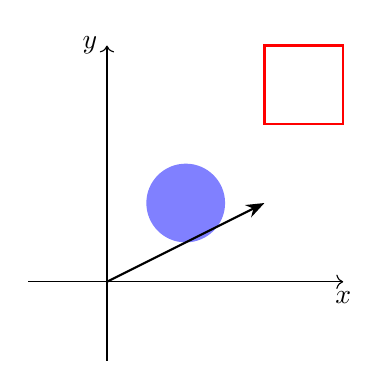
\begin{tikzpicture}
  % المحاور
  \draw[->] (-1,0) -- (3,0) node[below] {$x$};
  \draw[->] (0,-1) -- (0,3) node[left] {$y$};

  % دائرةٌ مملوءة
  \fill[blue!50] (1,1) circle (0.5);

  % مستطيلٌ بحدود
  \draw[thick, red] (2,2) rectangle (3,3);

  % سهمٌ من النقطةِ (0,0) إلى (2,1)
  \draw[-Stealth, thick] (0,0) -- (2,1);
\end{tikzpicture}

% عقدٌ موسومةٌ وأسهم
\begin{tikzpicture}[node distance=2cm]
  \node[draw, circle, fill=blue!20] (a) {$A$};
  \node[draw, rectangle, fill=red!20, right=of a] (b) {$B$};
  \node[draw, ellipse, fill=green!20, below=of b] (c) {$C$};

  \draw[->, thick] (a) -- (b);
  \draw[->, thick, dashed] (b) -- (c);
  \draw[->, thick, bend left] (a) to (c);
\end{tikzpicture}

\end{document}
